 \section{Overview: High-level components and their interaction}
A brief description of the general design context, the general approach and the overall design of the system with its processes is presented in this section of the DD.
\\Our system will be developed as a 4-tierrd JEE application, divided as Client Tier, Web Tier, Business Tier and the EIS Tier. %3-Tier???
\\The application is distributed over three locations: client machines, the Java EE server machine, and the database.
\\The mobile and web applications in particular are thin since data operations will be computed by a central server; in this way there is no heavy load on user side clients. We think that this is the most feasible approach because the two applications have the same goals. 


The diagram below provides a better understanding of the components of our system, highlighting the interactions in the architecture.
%\subsubsection{Architecture Component Diagram}
\begin{figure}[!h]
  \centering
  \vspace{0.2cm}
  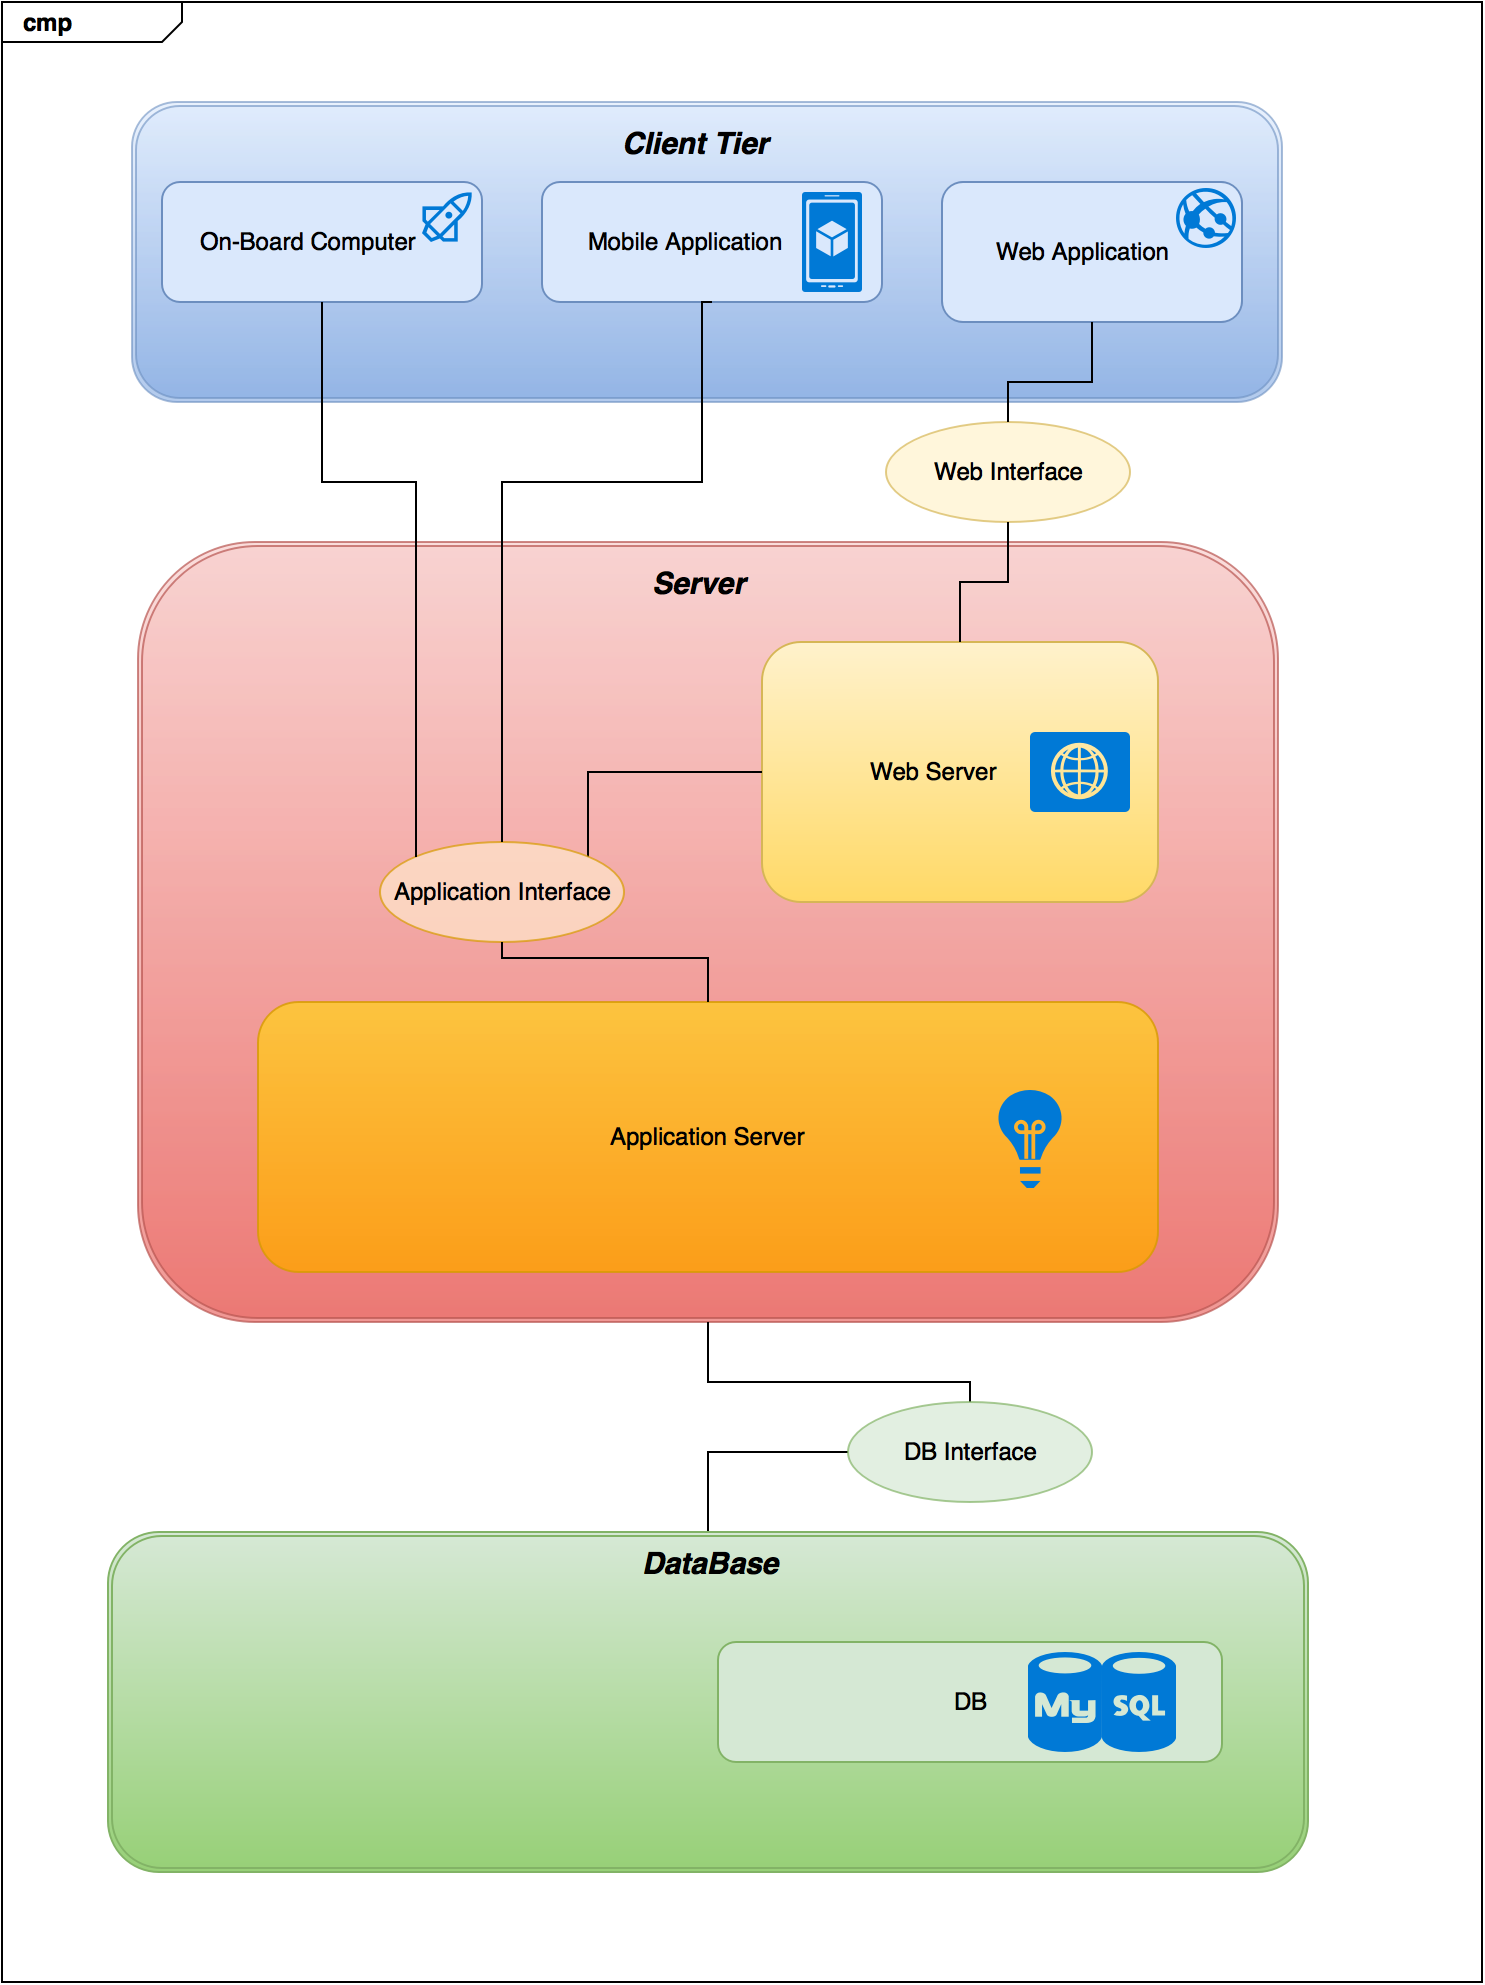
\includegraphics[width=0.6\textwidth]{/DD/4-Tier_Architecture}\\%TODO: add java beans and check the number of tiers
  \vspace{0.4cm}
  %\caption{Mockup for the login mobile page} 
  \label{fig:4-Tier_Architecture} 
\end{figure}

This represent a high level view of the design of the system, were is highlighted the distribution of the system over the three locations and the interaction between the different tiers thanks to their interfaces.
\\The Client Tier is composed by the On-board computer, the mobile application and the web application.
\\The Web Tier and the Business Tier are inside the server machine. We can observe that the Web application need to interact with the Web Server before to access to the Application server while the mobile application has a direct access to it.
\\The EIS Tier consists in a database that store all the system's data and interact through the DB Interface with the server.

 \section{Component view}
\subsection{System components}
To define and easily understand what kind of functionalities must be implemented in our system we decided to decompose PowerEnJoy logically into components. Then it is analysed each component and the interaction that it has with the other components, so the common parts can be identified if present. The components are studied to be reusable and easily adaptable in other applications.
%We have decided to decompose PowerEnJoy in different components in order to make it easy to understand what kind of functionalities must be implemented and to separate them, logically, in groups, to state clearer their interaction. The analysis of each component will give us the possibility to find common parts, if there are, and reuse them. 
\\The identified components are:
\begin{itemize}
	\item Access functionalities: provide sign-up to guests and log-in to users. They also allow credentials retrieving.
	\item Profile functionalities: provide the possibility for an user to modify her personal information.
	\item Reservation of the car: this functionality allows users to localize and reserve an available car.
	\item Ride functionalities: provide the possibility to unlock and lock of the car. Then all the system functions related with the ride are allocated here. %to change???
	\item Notification functionalities: provide the visualization of users' notifications, related to payments and reservations.%something else?
	\item Payments functionalities: provide the application of discounts or fees to a ride and menage the process related with the payments.
\end{itemize}

\subsection{Database components}
In particular the data stored in the database will be split through different subcomponents that identified the main entities of our system:
\begin{itemize}
	\item User  %location is not necessary, if a reservation is active we need a tag to indicate it
	\item Vehicle 
	\item SafaArea\&ChargingStation
	\item Reservation 
	\item Ride
	\item Payment  
	\item Notification 
\end{itemize} %something else??

The designed model for persistent data is provided here in a ER diagram in order to better analyze the motivations of our design. That's the representation of the database model:
\begin{figure}[!h]
  \centering
  \vspace{0.2cm}
  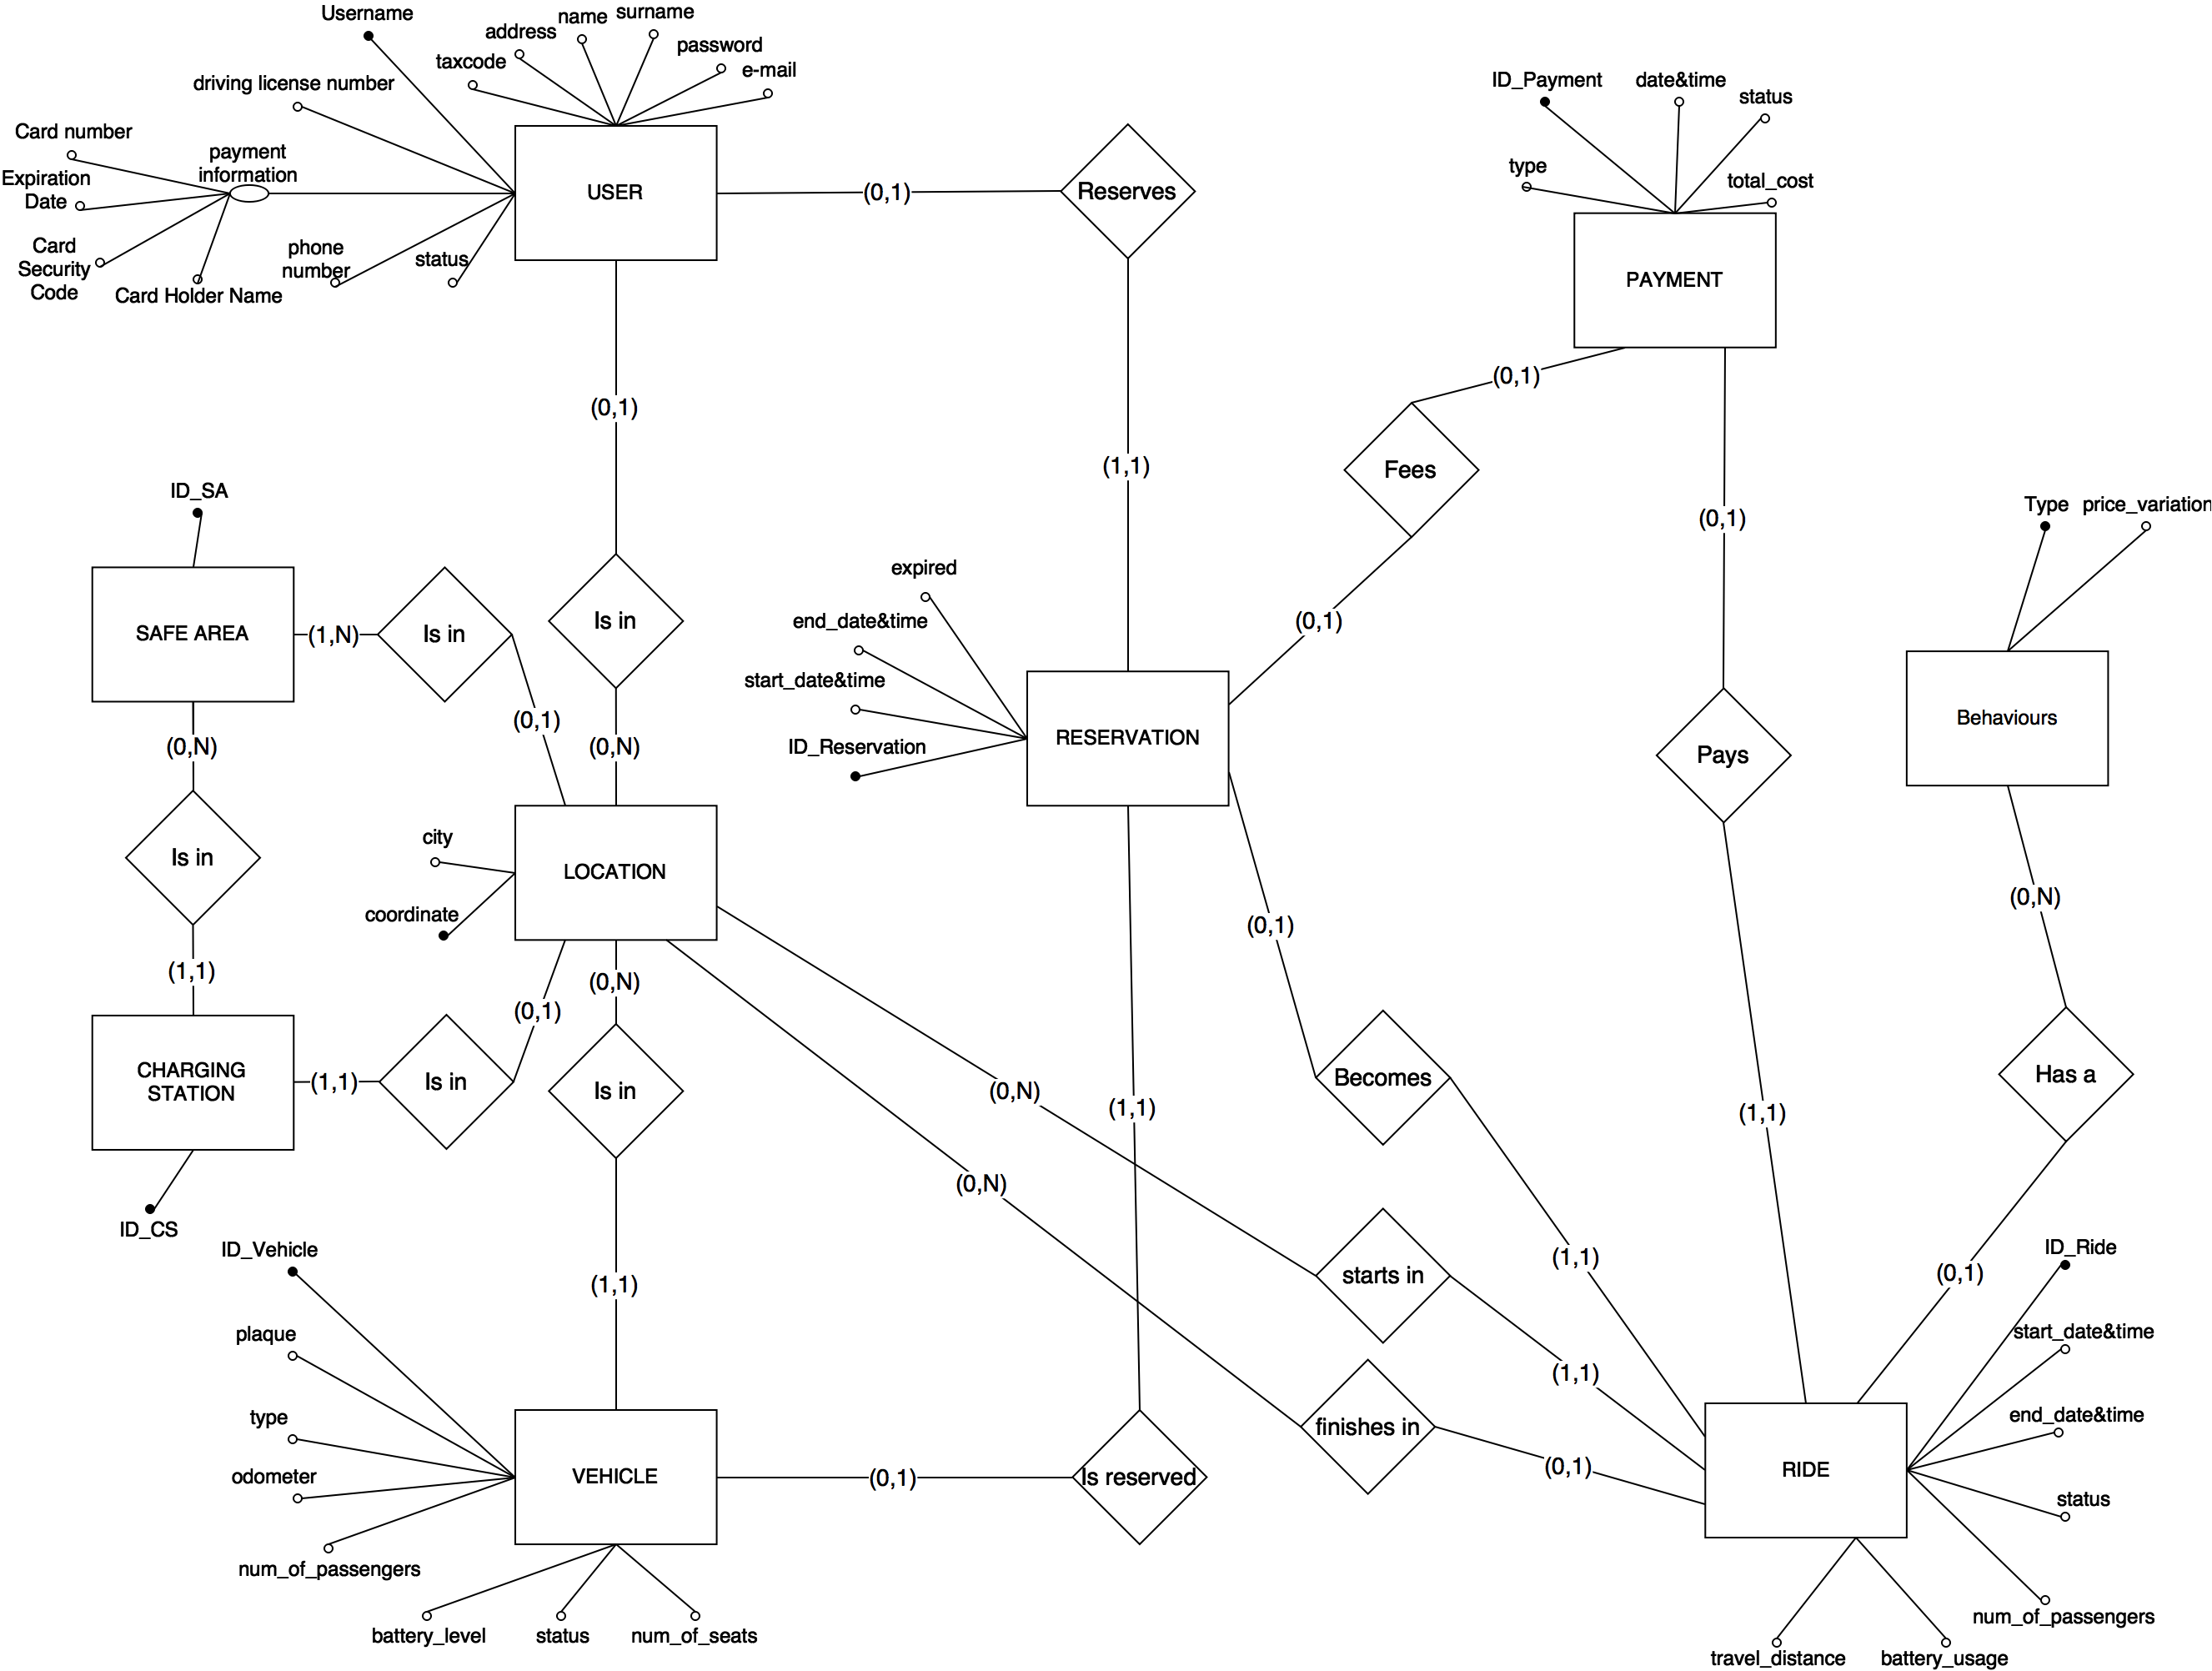
\includegraphics[width=0.7\textwidth]{/DD/ER_Diagram}\\%TODO: add java beans and check the number of tiers
  \vspace{0.4cm}
  %\caption{Mockup for the login mobile page} 
  \label{fig:ER_Diagram} 
\end{figure}

 And this is the relation schema associated with the ER diagram.
\begin{itemize} %TO CHECK WITH THE ER
	\item{User (\underline{ID\_User}, e-mail, pwd, driving\_license, name, surname, payment\_information, location, status)} %status: reserving, riding, free
	\item{Vehicle (\underline{ID\_Vehicle}, plaque, type, odometer, battery\_level, location, status, num\_of\_seats, num\_of\_passengers) }
	\item{SafaArea\&ChargingStation (\underline{location, type}, num\_of\_cars, city)} %type A=Safe Area, B=Charging Station, C=both
	\item{Reservation (\underline{ID\_reservation}, \textit{ID\_User}, \textit{ID\_Vehicle}, start\_date\&time, status)}
	\item{Ride (\underline{ID\_Ride}, \textit{ID\_User}, \textit{ID\_Vehicle}, \textit{ID\_Reservation}, \textit{ID\_Payment}, start\_date\&time, end\_date\&time, status, num\_of\_passengers, travel\_distance, star\_location, end\_location, battery\_usage )}
	\item{Payment (\underline{ID\_Payment}, \textit{ID\_User}, date\&time, total\_cost, fee\_or\_discount, final\_cost, status)}
	\item{Notification (\underline{ID\_Notification}, \textit{ID\_User}, type, date\&time, content)}
\end{itemize}

%TODO: write a little description of each entity, describing the attributes and the possible combinations

 \section{Deployment view}
The hardware topology is described here, highlighting components and their relationships. The software parts are deployed in or-
der to have the system working.
\\As previously see in the Overview the system will run thanks of 4 main components:
\begin{itemize}
	\item{The client device, where an User can interact with the system. There are different GUI that renders the web or mobile pages of our system, differentiating between On-board computer, mobile application and web application.}
	\item{ The Web Server is needed for those who are connected to the system with a computer. It establishes a secure internet connection through the HTTPS protocol.}
	\item{The Application Server is the core of our system. Here we have the Business Logic, where the whole system computation is
made.}
	\item{In the Database all the information of the system are stored. It's accessible only by the Application Server that store and take data from there.}
\end{itemize} 

%TO DO schema Deployment View

 \section{Runtime view}

In order to state the interaction between the different components of the system here are presented some sequence diagrams.
\\The sequence diagrams highlight the part of the system that interact for implement a function and the messages exchanged between them.
\\In this document are analyzed - different sequence diagrams: %decide the number
\begin{itemize}%TODO
	\item %TODO
\end{itemize} 



 \section{Component Interfaces}
 	\blindtext
 \section{Selected architectural styles and patterns}
